\documentclass[9pt, addpoints]{exam}

\usepackage[spanish]{babel}
\usepackage[utf8]{inputenc}
\usepackage[dvips]{graphicx}
\usepackage{amsmath}
\usepackage{amsfonts}
\usepackage{amssymb}
\usepackage{pifont}
\usepackage{multicol}
%\usepackage{psfrag}
\usepackage{color}
\usepackage{latexsym}
\usepackage{epsfig}
%\usepackage{pstricks}
%\usepackage[T1]{fontenc}
\usepackage{tikz}
\usepackage{bm}
\usepackage{bbold}

\usepackage[most]{tcolorbox}

% Language selection 
\newif\ifspanish
\spanishtrue % For the spanish version
\spanishfalse % For the english version

% Opción para las soluciones
\printanswers

\def\dunodcero{\begin{array}{c} D=1 \\ \gtrless \\ D=0 \end{array}}
\def\dceroduno{\begin{array}{c} D=0 \\ \gtrless \\ D=1 \end{array}}
\newcommand{\pfa}{P_{\text{FA}}} 
\newcommand{\pmis}{P_{\text{M}}} 
\newcommand{\pdet}{P_{\text{D}}} 
\newcommand{\EE}{\mathbb{E}} 

\newcommand{\ejMP}{
	\begin{tcolorbox}[boxrule=0.7pt, width=0.1\textwidth, left=2mm, right=0.1mm, top=0.1mm, bottom=0.1mm]
	\textbf{MP\thequestion} 
	\end{tcolorbox} ~~ \linefill }
\newcommand{\ejSP}{
	\begin{tcolorbox}[boxrule=0.7pt, width=0.1\textwidth, left=2mm, right=0.1mm, top=0.1mm, bottom=0.1mm]
	\textbf{SP\thequestion} 
	\end{tcolorbox} ~~ \linefill }

\hyphenation{im-pres-cin-di-ble}

\setlength{\textheight}{23cm} \setlength{\textwidth}{15cm}
\setlength{\marginparsep}{2mm} \setlength{\marginparwidth}{2cm}

\spanishdecimal{.}
\pointsinmargin
\marginpointname{\%}
\pagestyle{head}

%%%%%%%%%%
\ifspanish
\header{Procesos Estocásticos}{Problemas}{Curso Académico 2019/2020}
\else
\header{Stochastic Processes}{Problems}{Academic Year 2019/2020}
\fi

\headrule

\ifspanish
\title{{\bf Procesos Estocásticos: Problemas}}
\else
\title{{\bf Stochastic Processes: Problems}}
\fi


%%%%%%%%%%%%%%%%
\begin{document}

\maketitle

%%%%%%%%%%%%%%%%%%%%%%%%%%
\section{Markov Processes}
%%%%%%%%%%%%%%%%%%%%%%%%%%

%%%%%%%%%%%%%%%%%
\begin{questions}

%\qformat{\begin{tcolorbox}\textbf{\ej MP\thequestion ~~ (Markov Chain)}\end{tcolorbox}}
\qformat{\ejMP}
\question \ifspanish

TBD

\else

Let ${X_k, k \ge 0}$ be a Markov chain with state space ${\cal Z} = \{0, 1\}$ and transition probabilities $P\{X_k=1 | X_{k-1}=0\} = 0.8$ and $P\{X_k=0 | X_{k-1}=1\} = 0.4$.

\begin{parts}
\part Draw the corresponding transition graph
\part Assume that the initial state is  $X_0 = 1$. Compute $P\{X_2=1\}$
\part Compute the stationary distribution.
\end{parts}

\begin{solution}
\begin{parts}
\part The transition matrix is 
$$
{\bf P} = \begin{pmatrix}
0.2 & 0.8 \\
0.4 & 0.6
\end{pmatrix}
$$
and, thus, the transition graph is

{\centering
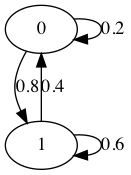
\includegraphics[scale=0.3]{db/figs/MPbinary.png}}

\part 
$$
P\{X_2=1\} = 
    \begin{pmatrix} 0 & 1 \end{pmatrix}
    {\bf P}^\intercal{\bf P}^\intercal
    \begin{pmatrix} 0 \\ 1 \end{pmatrix} 
    = 0.68
$$ 
\part The stationary distribution is the solution of
$$
{\bf P}^\intercal \boldsymbol{\pi} = \boldsymbol{\pi}
$$ 
with $(1, 1) \boldsymbol{\pi} = 1$, that is:
$$
0.2 \pi_0 + 0.4 \pi_1 = \pi_0
$$
and taking $\pi_1 = 1-\pi_0$, we get
$$
0.4 (1-\pi_0)  = 0.8 \pi_0
$$
so that $\pi_0 = \frac13$  and
$$
(\pi_0, \pi_1) = \left(\dfrac13, \dfrac23\right)
$$
\end{parts}
\end{solution}

\fi

\qformat{\ejMP}
\question \ifspanish
TBD
\else

Let ${X_k, k \ge 0}$ be a Markov chain with state space ${\cal Z} = \{0, 1, 2\}$ and the transition graph shown in the figure.
\begin{center}
\centering
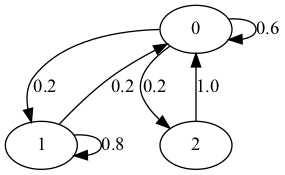
\includegraphics[width=0.25\textwidth]{./db/figs/MC_2023.png}
\end{center}

\begin{parts}
\part Show the transition matrix
\part Compute $P\{X_{22} = 1 | X_{20}=2\}$
\part Compute the stationary distribution.
\end{parts}

\begin{solution}
\begin{parts}
\part 
\begin{align*}
{\bf P} = 
	\begin{pmatrix}
	0.6 & 0.2 & 0.2   \\
	0.2 & 0.8 & 0     \\
	1   & 0   & 0 	
	\end{pmatrix}
\end{align*}
\part 
\begin{align*}
P\{X_{22} = 1| X_{20} = 2\} = 
	\begin{pmatrix} 0 & 1 & 0 \end{pmatrix}
	{\bf P}^\intercal
	{\bf P}^\intercal
	\begin{pmatrix} 0 \\ 0 \\ 1 	\end{pmatrix}
	=
	\begin{pmatrix} 0.2 & 0.8 & 0 \end{pmatrix}
	\begin{pmatrix} 1 \\ 0 \\ 0 \end{pmatrix}
	= 0.2
\end{align*}

\part This is the solution of
\begin{align*}
\begin{pmatrix}
{\bf P}^\intercal - {\bf I}  \\
\mathbb{1}^\intercal   
\end{pmatrix}
\bm{\pi} = 
\begin{pmatrix} 0 \\ 0 \\ 0 \\ 1 \end{pmatrix}
\end{align*}
that is
\textcolor{blue}{
\begin{align*}
\begin{pmatrix}
-0.4 &  0.2 &  0.2  \\
 0.2 & -0.2 &  0    \\
 0.2 &  0   & -1    \\
 1   &  1   &  1
\end{pmatrix}
\bm{\pi} = 
\begin{pmatrix} 0 \\ 0 \\ 0 \\ 1 \end{pmatrix}
\end{align*}}
which, removing the first row (which is redundant), reduces to
\textcolor{blue}{
\begin{align*}
\begin{pmatrix}
0.2  & -0.2 &  0    \\
0.2  & 0    & -1    \\
1    & 1    &  1
\end{pmatrix}
\bm{\pi} = 
\begin{pmatrix} 0 \\ 0 \\ 1 \end{pmatrix}
\end{align*}}
whose solution is
\begin{align*}
\bm{\pi} = 
\frac{1}{11} \begin{pmatrix} 5 \\ 5 \\ 1 \end{pmatrix}
\end{align*}

 \end{parts}
\end{solution}

\fi


\qformat{\ejMP}
\question \ifspanish

\else

Let ${X_k, k \ge 0}$ be a Markov chain with state space ${\cal Z} = \{0, 1, 2, 3\}$. The initial state is 0, that is, $P\{X_0=0\}=1$. If, at time $n$, the process is in state $i<3$, at time $n+1$ it will remain in the same state with probability $1-p$ or jump to state $i+1$ with probability $p$. 
\begin{align*}
P\{X_{n+1}=i+1 \mid X_n=i\} = p   \\
P\{X_{n+1}=i \mid X_n=i\} = 1-p
\end{align*}
If the process is in state 3, it will remain in the same state with probability 1.

\begin{parts}
\part Find the transition matrix
\part Show the transition graph
\part Compute $P\{X_2 = 1 \}$
\part Compute $P\{X_n = 0\}$, for any $n>0$
%\part Compute $P\{X_n = 3\}$, for any $n>0$
\part Find a stationary distribution for this process
\end{parts}

%%%%%%%%%%%%%%%%
\begin{solution}
\begin{parts}

\part
\begin{align*}
{\bf P} = 
	\begin{pmatrix}
	1-p & p   & 0   & 0   \\
	0   & 1-p & p   & 0   \\
	0   & 0   & 1-p & p   \\
	0   & 0   & 0   & 1 
	\end{pmatrix}
\end{align*}

\part
.
\begin{center}
\centering
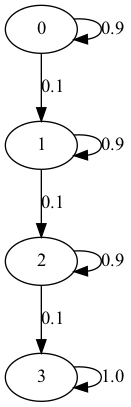
\includegraphics[width=0.1\textwidth]{./db/figs/P202306_markov_chain.png}
\end{center}

\part 
\begin{align*}
P\{X_2=1\} 
   &= \begin{pmatrix} 0 & 1 & 0 & 0 \end{pmatrix}
	  {\bf q}_2
    = \begin{pmatrix} 0 & 1 & 0 & 0\end{pmatrix}
	  {\bf P}^\intercal
	  {\bf P}^\intercal
	  \begin{pmatrix} 1 \\ 0 \\ 0 \\ 0 	\end{pmatrix}   \\
   &= \begin{pmatrix} p & 1-p & 0 & 0\end{pmatrix}
	  \begin{pmatrix} 1-p \\ p \\ 0 \\ 0 	\end{pmatrix}  
    = 2p (1-p) 
\end{align*}

\part $X_n=0$ if and only if there are no transitions from 0 to 1, that is $X_0=X_1=\ldots =X_n=1$. This will happen with probability
\begin{align*}
P\{X_n=0\} = (1-p)^n
\end{align*}
 
\part Eventually, the process will reach state 3 and remain there. Thus $\boldsymbol{\pi}=(0,0,0,1)$ must be a stationary distribution. Indeed,
\begin{align*}
{\bf P}^\intercal \boldsymbol{\pi} = 
	\begin{pmatrix}
	0   \\
	0   \\
	0   \\
	1 
	\end{pmatrix}
	= \boldsymbol{\pi}
\end{align*}


\end{parts}
\end{solution}


\fi

\qformat{\ejMP}
\question \ifspanish

Un videojuego consta de $N$ niveles consecutivos, $0, 1, ..., N-1$. El jugador empieza en el nivel 0. Si un jugador pasa el nivel $i$, entra en el nivel $i+1$, si no, vuelve al nivel 0. Se sabe que todas las fases tienen la misma dificultad, por lo que si jugador está en el nivel $i$, alcanza el nivel $i+1$ con probabilidad $q$, y regresa a 0 con probabilidad $1-q$.

Cuando el jugador alcanza la etapa $N-1$, obtiene una medalla, vuelve al nivel 0 y el juego continúa.

Sea $X_k$ el proceso estocástico que representa la secuencia de niveles durante un juego, tal que $X_k=i$ significa que el jugador estaba en el nivel $i$ en el momento $k$. El juego comienza en $X_0=0$.
\begin{parts}
\part Formule el problema como un proceso de Markov estacionario y dibuje el gráfico de transición para $N = 6$.
\part Asumiendo $N \ge 2$, calcule $P\{X_2=1\}$.
\part Suponiendo $N \ge 2$, determine la probabilidad de obtener una medalla exactamente en el tiempo $k$, es decir $P\{X_k=N-1\}$, para $k=0,1, \ldots, N$.
\part Para $N=2$, determine la distribución estacionaria.
\part Para $N=\infty$, determine la distribución estacionaria

\end{parts}

\begin{solution}
\begin{parts}
\part El grafo de transición se muestra en la figura para $q=0.1$.

{\centering
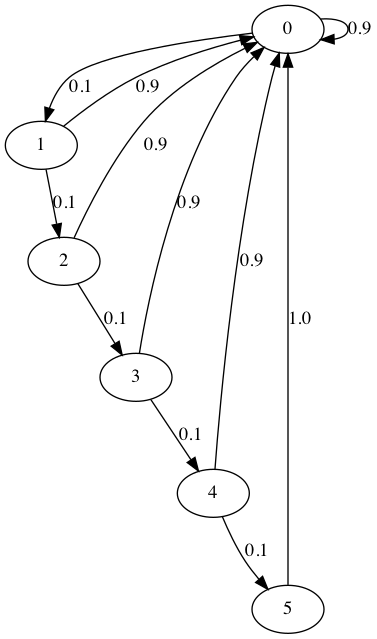
\includegraphics[scale=0.3]{db/figs/SPES_202106_markov_chain.png}}

\part 
\begin{align*}
P\{X_2=1\} = q P\{X_1=0\} = q (1-q) P\{X_0=0\} = q (1-q) 
\end{align*}

\part La probabilidad de obtener una medalla en el momento $k$ es $Q_k=P\{X_k=N-1\}$. Daddo que se requieren al menos $N-1$ pasos para alcanzar el nivel $N-1$, resulta
\begin{align*}
Q_k = 0,     \qquad \text{ for } k=0, \ldots, N-2
\end{align*}

Alcanzar el nivel $N-1$ en el momento $k=N-1$ is posible solamente si el jugador no falla en ninguna ocasión, de modo que
\begin{align*}
Q_{N-1} = q^{N-1}
\end{align*}

Alcanzar el nivel $N-1$ en $k=N$ es posible solamente si el jugador falla en el instante $0$ únicamente, de modo que
\begin{align*}
Q_{N} = (1-q) q^{N-1}
\end{align*}

\part Dado que
\begin{align*}
\pi_1 = q \pi_0
\end{align*}
y $\pi_0 + \pi_1 = 1$, resulta
\begin{align*}
\pi_1 = \frac{q}{1+q}
\end{align*}

\part Para $i>0$, se tiene que
\begin{align*}
\pi_i = q \pi_{i-1} = q^2 \pi_{i-2} = \ldots = q^i \pi_0
\end{align*}
y, para $i=0$,
\begin{align*}
\pi_0 = \sum_{i=0}^\infty (1-q) \pi_i 
       = (1-q) \sum_{i=0}^\infty \pi_i 
       = 1-q
\end{align*}
de modo que
\begin{align*}
\pi_i = (1-q) q^i
\end{align*}

\end{parts}
\end{solution}

\else

A video game consists of $N$ consecutive levels, $0, 1, ..., N-1$. The player starts at level 0. If a player passes level $i$, she enters level $i+1$, if not, she returns back to level 0. It is known that all phases have the same difficulty, so, if a player is at level $i$, she reaches level $i+1$ with probability $q$, and returns back to 0 with probability $1-q$. 

When the player reaches stage $N-1$, she gets a medal, returns to level 0 and the game continues.

Let $X_k$ be the stochastic process that represents the sequence of levels during a game, such that $X_k=i$ means that the player was at level $i$ at time $k$. The game begins at $X_0=0$.
\begin{parts}
\part Formulate the problem as a stationary Markov process, and draw the transition graph for $N = 6$.
\part Assuming $N \ge 2$, compute $P\{X_2=1\}$.
\part Assuming $N \ge 2$, determine the probability of obtaining a medal exactly at time $k$, that is $P\{X_k=N-1\}$, for $k=0,1, \ldots, N$.
\part For $N=2$, determine the stationary distribution.
\part For $N=\infty$, determine the stationary distribution

\end{parts}

\begin{solution}
\begin{parts}
\part The transition graph is shown in the figure for $q=0.1$.

{\centering
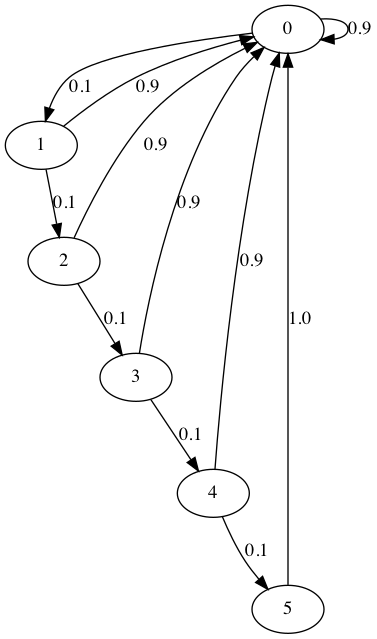
\includegraphics[scale=0.3]{db/figs/SPES_202106_markov_chain.png}}

\part 
\begin{align*}
P\{X_2=1\} = q P\{X_1=0\} = q (1-q) P\{X_0=0\} = q (1-q) 
\end{align*}

\part The probability of obtaining a medal at time $k$ is $Q_k=P\{X_k=N-1\}$. Since at least $N-1$ steps are required to reach level $N-1$, we have
\begin{align*}
Q_k = 0,     \qquad \text{ for } k=0, \ldots, N-2
\end{align*}

Reaching level $N-1$ at time $k=N-1$ is possible only if the player does not fail at any time, so that
\begin{align*}
Q_{N-1} = q^{N-1}
\end{align*}

Reaching level $N-1$ at time $k=N$ is possible only if the player fails at time $0$ only, so that.
\begin{align*}
Q_{N} = (1-q) q^{N-1}
\end{align*}

\part Since
\begin{align*}
\pi_1 = q \pi_0
\end{align*}
and $\pi_0 + \pi_1 = 1$, we have
\begin{align*}
\pi_1 = \frac{q}{1+q}
\end{align*}

\part For $i>0$, we have
\begin{align*}
\pi_i = q \pi_{i-1} = q^2 \pi_{i-2} = \ldots = q^i \pi_0
\end{align*}
and, for $i=0$,
\begin{align*}
\pi_0 = \sum_{i=0}^\infty (1-q) \pi_i 
       = (1-q) \sum_{i=0}^\infty \pi_i 
       = 1-q
\end{align*}
so that
\begin{align*}
\pi_i = (1-q) q^i
\end{align*}

\end{parts}
\end{solution}


\fi

\qformat{\ejMP}
\question 
\ifspanish

\else

A game has three players, named $G_0$, $G_1$ and $G_2$ and consists of a sequence of rounds. At each round, only one of the players enters the game. 

The result of each round can be win or lose. If the active player wins a round, she can play the next one. If she loses, she must pass the turn to one of the other players, which is chosen at random with equal probabilities.

Based on the game skills of the players, it is known that the winning probabilities are 0.4 (for $G_0$), 0.6 ($G_1$) and 0.8 ($G_2$).

Let $X_k$ be the one-sided stochastic process that represents the sequence of active players during a game, such that $X_k=i$ means that the active player at time $k$ is $G_i$.

The game always starts with player 0, that is, $X_0=0$.
\begin{parts}
\part [4] Formulate the problem as a stationary Markov chain: compute the transition matrix and draw the transition graph.
\part[4] Compute the probability that the first players in the sequence are $0, 1, 2, 1$ (i.e., $P\{X_0=0, X_1=1, X_2=2, X_3=1)$).
\part[5] Compute $P\{X_2=1\}$.
\part[5] Compute the stationary distribution
\part[5] Players $G_0$ and $G_1$ are unsatisfied because $G_2$, with better skills, plays most rounds. They decide to make the game fairer, in the sense that, in the long term, everyone plays with the same frequency. To do so, they proceed as follows: 
\begin{enumerate}
\item If $G_0$ is the active player and loses, she passes the turn to player $G_1$ with probability $q$ and to $G_2$ with probability $1-q$.
\item If $G_1$ is the active player and loses, she passes the turn to player $G_0$ with probability $r$ and to $G_2$ with probability $1-r$.
\end{enumerate}
Determine if $G_0$ and $G_1$ will succed in making a fair game, that is, if there exist values $q$ and $r$ so that the stationary distribution is uniform, i.e., $\boldsymbol{\pi}= (\frac13, \frac13, \frac13)$ If so, compute them.
\end{parts}

\begin{solution}
\begin{parts}
\part The transition matrix is
\begin{align*}
{\bf P} = \begin{pmatrix}
   0.4  & 0.3 & 0.3  \\
   0.2  & 0.6 & 0.2  \\
   0.1  & 0.1 & 0.8
\end{pmatrix}
\end{align*}
The transition graph is shown in the figure.

{\centering 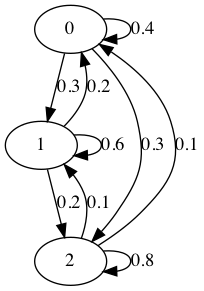
\includegraphics[scale=0.3]{db/figs/SP_202205_markov_chain.png}}

\part Since $X_k$ is a Markov chain
\begin{align*}
P\{X_0 &=0, X_1 =1, X_2=2, X_3=1\}   \\
	&= P\{X_0=0\} P\{X_1=1|X_0=0\} P\{X_2=2| X_1=1\} P\{X_3=1|X_2=2\}    \\
	&= 1 \cdot 0.3 \cdot 0.2 \cdot 0.1 = 0.006
\end{align*}

\part At time $k=2$, we have 
\begin{align*}
P\{X_2=1\} 
   &= \begin{pmatrix} 0 & 1 & 0 \end{pmatrix} 
      {\bf P}^\intercal {\bf P}^\intercal 
      \begin{pmatrix} 1 \\ 0 \\ 0 \end{pmatrix} 
    = \begin{pmatrix} 0.3 & 0.6 & 0.1 \end{pmatrix} 
      \begin{pmatrix} 0.4 \\ 0.3 \\ 0.3 \end{pmatrix} 
%    = 0.12 + 0.18 + 0.03 
    = 0.33
\end{align*}

\part The stationary distribution is the solution of
\begin{align*}
\begin{pmatrix}
   0.4 & 0.2 & 0.1 \\
   0.3 & 0.6 & 0.1 \\
   0.3 & 0.2 & 0.8 \\
   1   & 1   & 1 
\end{pmatrix}
\begin{pmatrix} \pi_0 \\ \pi_1 \\ \pi_2 \end{pmatrix} = 
\begin{pmatrix} \pi_0 \\ \pi_1 \\ \pi_2  \\ 1 \end{pmatrix}
\end{align*}
Since the first 3 equations are linearly dependent, we can remove the first one, 
\begin{align*}
\begin{pmatrix}
   1   &  1   & 1  \\
   0.3 & -0.4 & 0.1  \\
   0.3 &  0.2 & -0.2
\end{pmatrix}
\begin{pmatrix} \pi_0 \\ \pi_1 \\ \pi_2 \end{pmatrix} = 
\begin{pmatrix} 1     \\ 0     \\ 0     \end{pmatrix}
\end{align*}
%which is equivalent to
%\begin{align*}
%\begin{pmatrix}
%   1 &  1   &  1   \\
%   0 & -0.7 & -0.2 \\
%   0 & -0.1 & -0.5 
%\end{pmatrix}
%\begin{pmatrix} \pi_0 \\ \pi_1 \\ \pi_2 \end{pmatrix} = 
%\begin{pmatrix} 1     \\ -0.3  \\ -0.3  \end{pmatrix}
%\end{align*}
%which is equivalent to
%\begin{align*}
%\begin{pmatrix}
%   1 & 1   & 1   \\
%   0 & 0.1 & 0.5 \\
%   0 & 0.7 & 0.2
%\end{pmatrix}
%\begin{pmatrix} \pi_0 \\ \pi_1 \\ \pi_2 \end{pmatrix} = 
%\begin{pmatrix} 1     \\ 0.3   \\ 0.3   \end{pmatrix}
%\end{align*}
%which is equivalent to
%\begin{align*}
%\begin{pmatrix}
%   1 &  1   & 1   \\
%   0 &  0.1 & 0.5 \\
%   0 &  0   & -3.3
%\end{pmatrix} 
%\begin{pmatrix} \pi_0 \\ \pi_1 \\ \pi_2 \end{pmatrix} = 
%\begin{pmatrix} 1     \\ 0.3   \\ -1.8  \end{pmatrix}
%\end{align*}
Therefore:
\begin{align*}
\begin{pmatrix} \pi_0 \\ \pi_1 \\ \pi_2 \end{pmatrix} = 
\frac{1}{11}
\begin{pmatrix} 2 \\ 3 \\ 6 \end{pmatrix}
\end{align*}

\part If the stationary distribution is uniform, we have
\begin{align*}
\begin{pmatrix}
   0.4       & 0.4 r    & 0.1 \\
   0.6 q     & 0.6      & 0.1 \\
   0.6 (1-q) & 0.4(1-r) & 0.8
\end{pmatrix}
\begin{pmatrix} \tfrac13 \\ \tfrac13 \\ \tfrac13 \end{pmatrix} = 
\begin{pmatrix} \tfrac13 \\ \tfrac13 \\ \tfrac13 \end{pmatrix}
\end{align*}
Using the first to equations, we have
\begin{align*}
0.4   + 0.4 r + 0.1 = 1  \\
0.6 q + 0.6   + 0.1 = 1
\end{align*}
The unique solution is $q=0.5$, $r=1.25$. Since $r$ is not a probability value, there is no way to make the game fair.

\end{parts}
\end{solution}


\fi

\end{questions}

%%%%%%%%%%%%%%%%%%%%%%%%%%%%%%%
\section{Stationary Processes}
%%%%%%%%%%%%%%%%%%%%%%%%%%%%%%%

%%%%%%%%%%%%%%%%%
\begin{questions}

\qformat{\ejSP}
\question \ifspanish

TBD

\else

Let $X_n$ be i.i.d. stochastic process with probability density function
\[
p_{X}(x) = x \exp(-x), \qquad x \ge 0
\]

Assume that $X_n$ is the input to a linear system with impulse response
\[
h_n = \delta[n] + 0.5 \delta[n-1]
\]
the system output $Y_n$, is corrupted by a Gaussian i.i.d noise $E_n$ (independent of $X_n$) with mean zero and unit variance, to produce the final process
\[
Z_n =  Y_n + E_n
\]

\begin{parts}
\part Compute the autocorrelation functions $r_X[n]$ and $r_E[n]$ of $X_n$ and $E_n$, respectively.
\part Compute the autocorrelation function of $Y_n$,  $r_Y[n]$
\part Compute the autocorrelation function of $Z_n$,  $r_Z[n]$
\part Compute the power spectrum of $Z_n$, $S_Z(\omega)$..
\end{parts}

\begin{solution}
\begin{parts}
\part 
Since $X_n$ is zero-mean i.i.d, we have
\begin{align*}
r_X[n] 
	&= \EE	\{X_k X_{k+n} \} = 
       \left[
	   \begin{array}{ll}
	   \EE\{X_k^2\},            & n=0 \\
	   \EE\{X_k\}\EE\{X_{k+n}\}, & n \neq 0	
	   \end{array}
	   \right. \\
	&= \EE\{X_k^2\} \delta[n] + \EE\{X_k\}^2 (1-\delta[n])   \\
	&= \left(\EE\{X_k^2\} - \EE\{X_k\}^2\right) \delta[n] + \EE\{X_k\}^2
\end{align*}
Noting that
\begin{align*}
\EE\{X_k\}   &= \int_0^\infty x^2 \exp(-x)dx = 2  \\
\EE\{X_k^2\} &= \int_0^\infty x^3 \exp(-x)dx = 6
\end{align*}
we get
\begin{align*}
r_X[n] = 2 \delta[n] + 4
\end{align*}

Since $E_n$ is zero-mean i.i.d, we have
\begin{align*}
r_E[n] = \sigma_E^2 \delta[n] = \delta[n]
\end{align*}

\part Since
\begin{align*}
Y_n = X_n \ast h_n 
\end{align*}
we have
\begin{align*}
r_Y[n] 
	&= r_X[n] \ast h_n \ast h_{-n} \\
	&= (2 \delta[n] + 4) \ast (\delta[n] + 0.5\delta[n-1]) \ast (\delta[n] + 0.5\delta[n+1]) \\
	&= (2 \delta[n] + 4) \ast (1.25 \delta[n] + 0.5\delta[n-1] + 0.5\delta[n+1]) \\
	&= 2.5 \delta[n] + \delta[n-1] + \delta[n+1] + 9
\end{align*}

\part Since $Y_n$ and $E_n$ are independent and $E_n$ is zero-mean
\begin{align*}
r_Z[n] = r_Y[n] + r_E[n] = 3.5 \delta[n] + \delta[n-1] + \delta[n+1] + 9
\end{align*}

\part Computing the Fourier transform of the autocorrelation function, we get
\begin{align*}
S_Z(\omega) = 3.5 + 2 \cos(\omega) + 18 \pi \delta(\omega),    \qquad \omega \in [-\pi, \pi]
\end{align*}

\end{parts}
\end{solution}

\fi

\qformat{\ejSP}
\question \ifspanish

\else

The stochastic process  $X_n$ is given by,
\[X_n = \exp\left(- S_n \right)\]
where $S_n$ is an i.i.d. process with probability density function
\[p_S(s) = \lambda \exp(- \lambda s),  \qquad s \ge 0, \qquad \lambda > 0\]
Assume that $X_n$ is the input to a linear and time-invariant system with impulse response
\[h[n] = \delta[n] - \delta[n-1]\]
with output $Y_n$

\begin{parts}
\part Compute the mean of the process, $\mu_X = \mathbb{E}\{X_n\}$.
\part Compute the autocorrelation function, $r_X[n]$.
\part Compute the power spectrum of the process $Y_n$ for $\lambda=1$
\end{parts}

\begin{solution}
\begin{parts}
\part The mean is given by
\begin{align*}
\mu_X &= \mathbb{E}\{\exp(-S_n)\} 
       = \int_{-\infty}^{\infty} \exp(- s) \cdot p_S(s) ds 
       = \int_0^{\infty} \exp(- s) \cdot \lambda  \exp(- \lambda s) ds    \\
      &= \lambda  \int_0^{\infty} \exp(- (\lambda+1) s) ds = \frac{\lambda}{\lambda+1}
\end{align*}
\part Since $X_k$ is i.i.d., the autocorrelation is
\begin{align*}
r_X[n] &= \mathbb{E}\{X_k X_{k+n}\} 
        = \left[\begin{array}{ll}
            \mathbb{E}\{X_k\} \mathbb{E}\{X_{k+n}\},    & n \neq 0 \\ 
       		\mathbb{E}\{X_k^2\},                 & n = 0
       	  \end{array}\right.
\end{align*}
Noting that
\begin{align*}
\mathbb{E}\{X_k^2\} 
    &= \mathbb{E}\{\exp(-2S_n)\} 
     = \lambda  \int_0^{\infty} \exp(- (\lambda+2) s) ds
     =\frac{\lambda}{\lambda+2}
\end{align*}
we get
\begin{align*}
r_X[n] &= \mathbb{E}\{X_k X_{k+n}\} 
        = \left[\begin{array}{ll}
            \frac{\lambda^2}{(\lambda+1)^2},    & n \neq 0 \\ 
       		\frac{\lambda}{\lambda+2},                 & n = 0
       	  \end{array}\right.
\end{align*}
\part 
For $\lambda=1$, we get
\begin{align*}
r_X[n] &= \left[\begin{array}{ll}
            \frac{1}{4},      & n \neq 0 \\ 
       		\frac{1}{3},      & n = 0
       	  \end{array}\right]
       	=  \frac{1}{4} + \frac{1}{12} \delta[n]
\end{align*}
therefore
\begin{align*}
S_X(\omega) 
	&= \frac{\pi}{2} \delta(\omega) + \frac{1}{12}, \qquad \qquad  -\pi \le \omega \le \pi
\end{align*}
and
\begin{align*}
S_Y(\omega) 
	&= S_X(\omega) |H(\omega)|^2
	 = \left( \frac{\pi}{2} \delta(\omega) + \frac{1}{12} \right) |1 - \exp(-j\omega)|^2 \\
	&= \frac{1}{12} |1 - \exp(-j\omega)|^2
	 = \frac{1}{6} (1 - \cos(\omega))
\end{align*}

(Alternatively, we can also compute $S_Y(\omega)$ from $r_X[n]$ through $r_Y[n]$:
\begin{align*}
r_Y[n] &= r_X[n]  \ast h[n] \ast h[-n]   \\
       &= r_X[n]  \ast (\delta[n]-\delta[n-1]) \ast (\delta[-n]-\delta[-n-1]) \\
       &= r_X[n]  \ast (\delta[n]-\delta[n-1]) \ast (\delta[n]-\delta[n+1])   \\
       &= r_X[n]  \ast (2\delta[n]-\delta[n-1]-\delta[n+1]) \\
       &= (2 r_X[n] -r_X[n-1]-r_X[n+1]) \\
       &= \frac{1}{12} (2  \delta[n] -  \delta[n-1] - \delta[n+1])
\end{align*}
and, applying the Fourier transform,
\begin{align*}
S_Y(\omega) 
	&= \frac{1}{12} \left(2 - e^{-j\omega} - e^{j\omega}\right)
	 = \frac{1}{6} (1 - \cos(\omega))
\end{align*}

 
\end{parts}
\end{solution}

\fi

\qformat{\ejSP}
\question % JCS

\ifspanish

El proceso estocástico $X_n$ viene dado por el par de ecuaciones
\begin{align*}
X_n &= S_n \cdot R_n \\
S_n &= W_n - \frac12 W_{n-1}
\end{align*}
donde $W_n$ es un proceso i.i.d. gausiano con media $0$ y varianza $v$, y $R_n$ es un proceso estacionario con función de autocorrelación
\begin{align*}
r_R[n] = 2^{-|n|}
\end{align*}
Los procesos $W_n$ y $R_n$ son independientes entre sí.
\begin{parts}
\part Calcule la función de autocorrelación de $W_n$, $r_W[n]$
\part Calcule y dibuje la función de autocorrelación de $S_n$, $r_S[n]$
\part Calcule y dibuje la función de autocorrelación de $X_n$, $r_X[n]$
\part Calcule el espectro de potencia del proceso $Z_n = \sum_{k=0}^\infty 2^{-k} X_{n-k}$
\end{parts}

\begin{solution}
\begin{parts}
\parte
\begin{align*}
r_W[n] = v \delta[n]
\end{align*}
\parte
\begin{align*}
r_S[n] &= \mathbb{E}\{S_k \cdot S_{k+n}\} \\
       &= \mathbb{E}\{(W_k - \frac12 W_{k-1})(W_{k+n} - \frac12 W_{k+n-1})\} \\
       &= \frac{5}{4} v \delta[n] - \frac12 v \delta[n-1] - v \frac12 \delta[n+1] \\
\end{align*}
\parte
\begin{align*}
r_X[n] &= \mathbb{E}\{X_k \cdot X_{k+n}\} \\
       &= \mathbb{E}\{S_k \cdot S_{k+n}\} \mathbb{E}\{R_k \cdot R_{k+n}\} \\
       &= r_S[n] r_R[n] \\
       &= 2^{-|n|} \cdot
          \left(\frac{5}{4} v \delta[n] - \frac12 v \delta[n-1] - v \frac12 \delta[n+1]\right) \\
       &= \frac{5}{4} v \delta[n] - \frac14 v \delta[n-1] - \frac14 v \delta[n+1])
\end{align*}
\parte
\begin{align*}
Z_n &= X_n \ast h[n]
\end{align*}
donde $h_n = 2^{-n} u[n]$. Por lo tanto
\begin{align*}
S_Z(\omega) 
     &= S_X(\omega) |H(\omega)|^2 \\
     &= \frac{v}{2} \left(\frac52 - \cos(\omega)\right) \left|\frac{1}{1-\frac12 \exp(-j\omega)}\right|^2   \\
     &= \frac{v}{2} \cdot \frac{\frac52 - \cos(\omega)}{ \left|1-\frac12 \exp(-j\omega)\right|^2}  \\
     &= v \cdot \frac{5 - 2 \cos(\omega)}{5 - 4\cos(\omega)}
\end{align*}
\end{parts}
\end{solution}

\else

The stochastic process  $X_n$ is given by the  pair of equations
\begin{align*}
X_n &= S_n \cdot R_n   \\
S_n &= W_n - \frac12 W_{n-1}
\end{align*}
where $W_n$ is a Gaussian i.i.d. process with mean $0$ and variance $v$, and $R_n$ is stationary processes with autocorrelation function
\begin{align*}
r_R[n] = 2^{-|n|} 
\end{align*}
Processes $W_n$ and $R_n$ are mutually independent.

\begin{parts}
\part Compute the autocorrelation function of $W_n$, $r_W[n]$
\part Compute and draw the autocorrelation function of $S_n$, $r_S[n]$
\part Compute and draw the autocorrelation function of $X_n$, $r_X[n]$
\part Compute the power spectrum of the process $Z_n = \sum_{k=0}^\infty 2^{-k} X_{n-k}$
\end{parts}


\begin{solution}
\begin{parts}
\part Since $W_n$ is zero-mean i.i.d, $r_W[n] = v \delta[n]$
\part 
\begin{align*}
r_S[n] &= \mathbb{E}\{S_k \cdot S_{k+n}\}   \\
       &= \mathbb{E}\{(W_k - \frac12 W_{k-1})(W_{k+n} - \frac12 W_{k+n-1})\} \\
       &= \frac{5}{4} v \delta[n] - \frac12 v \delta[n-1] - v \frac12 \delta[n+1] 
\end{align*}
\part
\begin{align*}
r_X[n] &= \mathbb{E}\{X_k \cdot X_{k+n}\}   \\
       &= \mathbb{E}\{S_k \cdot S_{k+n}\} \mathbb{E}\{R_k \cdot R_{k+n}\}  \\
       &= r_S[n] r_R[n]   \\
       &= 2^{-|n|} \cdot
          \left(\frac{5}{4} v \delta[n] - \frac12 v \delta[n-1] - v \frac12 \delta[n+1]\right) \\
       &= \frac{5}{4} v \delta[n] - \frac14 v \delta[n-1] - \frac14 v \delta[n+1]) 
\end{align*}
\part
\begin{align*}
Z_n &= X_n \ast h[n]
\end{align*}
where $h_n = 2^{-n} u[n]$. Therefore
\begin{align*}
S_Z(\omega) 
     &= S_X(\omega) |H(\omega)|^2 \\
     &= \frac{v}{2} \left(\frac52 - \cos(\omega)\right) \left|\frac{1}{1-\frac12 \exp(-j\omega)}\right|^2   \\
     &= \frac{v}{2} \cdot \frac{\frac52 - \cos(\omega)}{ \left|1-\frac12 \exp(-j\omega)\right|^2}  \\
     &= v \cdot \frac{5 - 2 \cos(\omega)}{5 - 4\cos(\omega)}
\end{align*}

\end{parts}
\end{solution}

\fi


\qformat{\ejSP}
\question \ifspanish

TBD

\else

The stochastic process  $X_n$ is the sum of two i.i.d. stochastic processes $S_n$ and $R_n$,
\[
X_n = S_n + R_n
\]
with probability density functions
\[
p_{S}(s) = s \exp(-s), \qquad s \ge 0
\]
and
\[
p_{R}(r) = \frac{1}{\sqrt{2\pi}} \exp\left(-\frac{r^2}{2} \right)
\]
respectively. The processes $S_n$ and $R_n$ are mutually independent. Assume that $X_n$ is the input to a linear and time-invariant system with impulse response
\[
h_n = \frac1{2^n} u[n]
\]
with output $Y_n$

\begin{parts}
\part Compute the autocorrelation function, $r_X[n]$, and the power spectrum, $S_X(\omega)$, of $X_n$
\part Compute the autocorrelation function, $r_Y[n]$, and the power spectrum, $S_Y(\omega)$, of $Y_n$
\end{parts}

\begin{solution}
\begin{parts}
\part 
\begin{align*}
r_X[n] &= \mathbb{E}\{X_k X_{k+n}\}   \\
       &= \mathbb{E}\{(S_k + R_k) (S_{k+n} + R_{k+n}) \}   \\
       &= r_S[n] + r_R[n] + \mathbb{E}\{S_k\} \mathbb{E}\{R_{k+n}\} + \mathbb{E}\{R_k\} \mathbb{E}\{S_{k+n}\}   \\
       &= r_S[n] + r_R[n]
\end{align*}
Since $S_n$ and $R_n$ are i.i.d.
\begin{align*}
r_S[n] &= \mathbb{E}\{S_k S_{k+n}\}   \\
       &= \mathbb{E}\{S_k^2\} \delta[n] + \mathbb{E}\{S_k\} \mathbb{E}\{S_{k+n}\} (1-\delta[n])    \\
       &= \int_0^\infty s^3 \exp(-s) ds \cdot \delta[n] + \left(\int_0^\infty s^2 \exp(-s) ds\right)^2 (1-\delta[n])   \\
       &= 3! \delta[n] + 4 (1-\delta[n])   \\
       &=  4 + 2 \delta[n]   
\end{align*}
and
\begin{align*}
r_R[n] &= \mathbb{E}\{R_k R_{k+n}\}   \\
       &= \mathbb{E}\{R_k^2\} \delta[n] + \mathbb{E}\{R_k\} \mathbb{E}\{R_{k+n}\} (1-\delta[n])   
        = \delta[n]  
\end{align*}
Therefore
\begin{align*}
r_X[n] &= 4 + 3 \delta[n] 
\end{align*}
and the power spectrum is
\begin{align*}
S_X(w) &= 3 + 8\pi \delta(\omega),   \qquad\qquad  -\pi \le \omega \le \pi 
\end{align*}
\part 
\begin{align*}
r_Y[n] &= r_X[n] \ast h[n] \ast h[-n]    \\
       &= \frac{4}{3} \left(\frac{1}{2}\right)^{-|n|} \ast (4 + 3 \delta[n]) 
        = 16 + 4 \left(\frac{1}{2}\right)^{-|n|} \\
S_Y(w) &= S_X(w) |H(\omega)|^2     \\
        &= \frac{3 + 8 \pi \delta(\omega)}{\left|1 - \frac12 e^{-j\omega} \right|^2}
\end{align*}
(This expression can be further simplified to
\begin{align*}
S_Y(w) &= \frac{3 + 8\pi \delta(\omega)}{\frac54 - \cos(\omega)}
        = \frac{3}{\frac54 - \cos(\omega)} + 32 \pi \delta(\omega)
\end{align*}
). 

\end{parts}
\end{solution}

\fi

\qformat{\ejSP}
\question \ifspanish

\else

Let $X_n$ be a discrete two-sided IID process with probability density function
\begin{align*}
p_X(x) = \frac12,  \qquad -1 \le x \le 1
\end{align*}

Let $Y_n$ be the process defined by
\begin{align*}
Y_n = X_n^3
\end{align*}

Let $Z_n$ be the output of a linear time-invariant filter with impulse response:
\begin{align*}
h[n] = \frac{u[n]}{3^n} 
\end{align*}
when the input is $Y_n$. 

\begin{parts}
\part Is $X_n$ wide-sense-stationary (WSS)? Is it strict-sense stationary (SSS)?

\part Compute the mean $\mu_Y[n]$ and the autocorrelation function, $r_Y[n]$, of $Y_n$.

\part Compute the power spectrum of $Z_n$, $S_Z\left(e^{j\omega}\right)$

\part Find the impulse response $g[n]$ of a linear-time invariant system such that, if $V_n$ is the output of the system for input $Z_n$, the autocorrelation function of $V_n$ is
\begin{align*}
r_V[n] = \delta[n] 
\end{align*}

\end{parts}

\begin{solution}
\begin{parts}
\part Since $X_n$ is IID, it is WSS and SSS.
\part
\begin{align*}
\mu_Y[n] 
	= \mathbb{E}\{Y_n\} 
	= \mathbb{E}\{X_n^3\} 
	= \frac12 \int_{-1}^1 x^3 dx = 0
\end{align*}
\begin{align*}
r_Y[n] 
	&= \mathbb{E}\{Y_m Y_{m+n}\}
	= \left[\begin{array}{ll}
		\mathbb{E}\{X_m^6\},                           & n = 0,    \\	
		\mathbb{E}\{X_m^3\} \mathbb{E}\{X_{m+n}^3\},   & n \neq 0, \\	
	  	\end{array}
	  \right.  \\
	&= \mathbb{E}\{X_m^6\} \delta[n]
	 = \frac12 \int_{-1}^1 x^6 dx \delta[n] 
	 = \frac17 \delta[n]
\end{align*}
\part
\begin{align*}
S_Z\left(e^{j\omega}\right) 
	=& S_Y\left(e^{j\omega}\right) \left| H\left(e^{-j\omega}\right) \right|^2   \nonumber\\
	=& \frac{1}{7 \left| 1 - \frac13 e^{-j\omega}\right|^2}
\end{align*}
\part 
If the autocorrelation is $r_V[n] = \delta[n]$, the power spectrum is $S_V\left(e^{j\omega}\right) = 1$. Since
\begin{align*}
S_V\left(e^{j\omega}\right) = S_Z\left(e^{j\omega}\right) \left|G\left(e^{j\omega}\right)\right|^2
\end{align*}
we have 
\begin{align*}
\frac{1}{7 \left| 1 - \frac13 e^{-j\omega}\right|^2} \left|G\left(e^{j\omega}\right)\right|^2 = 1
\end{align*}
therefore
\begin{align*}
\left|G\left(e^{j\omega}\right)\right|^2 = 7 \left| 1 - \frac13 e^{-j\omega}\right|^2
\end{align*}
that is
\begin{align*}
G\left(e^{j\omega}\right)G^*\left(e^{j\omega}\right) = 7 \left(1 - \frac13 e^{-j\omega}\right)\left(1 - \frac13 e^{j\omega}\right)
\end{align*}
Therefore, we can take, for instance
\begin{align*}
G\left(e^{j\omega}\right) = \sqrt{7} \left(1 - \frac13 e^{-j\omega}\right)
\end{align*}
so that
\begin{align*}
g[n] = \sqrt{7} \left(\delta[n] - \frac13 \delta[n-1]\right)
\end{align*}

\end{parts}
\end{solution}

\fi

\qformat{\ejSP}
\question \ifspanish

\else

Suppose that $X_n$ is a two-sided binary Bernoulli($p$) process, that is, an IID process given by
\begin{align*}
P_{X_n}(k) 
	&= \left[\begin{array}{ll}
             p,   &  k=1   \\
             1-p, &  k=0
          \end{array} \right]   % \\
%	&= p^k (1-p)^{1-k},     \qquad\qquad  0 \le p \le 1, \qquad i\in \{0,1\}, \qquad n \in \mathbb{Z}
,   \qquad\qquad n\in \mathbb{Z}
\end{align*}

Using $X_n$, we define the following random processes
\begin{align*}
T_n &= X_n \cdot X_{n-1}      \\
U_n &= X_n \cdot X_{n-1}, \cdots X_{n-\ell},    \qquad m \ge 1
\end{align*}
where operator $\oplus$ denotes mod 2 addition

\begin{parts}
\part Compute the probability mass function of $T_n$, $P_{T_n}(k)$, $k\in\{0, 1\}$.
\part Compute the autocorrelation function, $r_T[n]$, of $T_n$.
\part Compute the power spectrum of $T_n$, $S_T(\omega)$.
\part Compute the probability mass function of $U_n$, $P_{U_n}(k)$, $k\in\{0, 1\}$.
\part Compute the autocorrelation function, $r_U[n]$, of $U_n$.
\end{parts}

\begin{solution}
\begin{parts}

\part
\begin{align*}
P_T(1) &= P\{X_n=1, X_{n-1}=1\} = p^2  \\
P_T(0) &= 1-p^2
\end{align*}

\part For $T_n$ we have
\begin{align*}
r_T[n] &= \mathbb{E}\{T_m T_{m+n}\}   \\
       &= \left[\begin{array}{ll}
             \mathbb{E}\{X_m^2 X_{m-1}^2 \},                        &  n=0         \\
             \mathbb{E}\{X_{m-1} \cdot X_m^2 \cdot X_{m+1}\},         &  n\in \{-1, 1\}  \\
             \mathbb{E}\{X_{m-1} \cdot X_m \cdot X_{m+n-1} \cdot X_{m+n} \},  &  |n| > 1
          \end{array} \right.
\end{align*}
and, noting that, since $X_m$ is a binary process, $X_m^2=X_m$,
\begin{align*}
r_T[n] &= \mathbb{E}\{T_m T_{m+n}\}   \\
       &= \left[\begin{array}{ll}
             \mathbb{E}\{X_m \} \mathbb{E}\{X_{m-1} \},              &  n=0         \\
             \mathbb{E}\{X_{m-1}\} \cdot \mathbb{E}\{X_m\} \cdot \mathbb{E}\{X_{m+1}\},    &  n\in \{-1, 1\}  \\
             \mathbb{E}\{X_{m-1}\} \cdot \mathbb{E}\{X_m\} \cdot \mathbb{E}\{X_{m+n-1}\} 
             \mathbb{E}\{X_{m+n}\},  &  |n| > 1
          \end{array} \right.   \\
       &= \left[\begin{array}{ll}
             p^2,   &  n=0   \\
             p^3,   &  n \in \{-1, 1\}   \\
             p^4,   &  |n| > 1
          \end{array} \right.   \nonumber\\
       &= (p^2 -p^4)\delta[n] + (p^3 -p^4)\left(\delta[n-1] + \delta[n+1]\right) + p^4 
\end{align*}
\part 
The power spectrum is 
\begin{align*}
S_T(\omega) &= (p^2 -p^4)  + 2 (p^3 -p^4) \cos(\omega) + 2\pi p^4 \delta(\omega)
\end{align*}

\part
\begin{align*}
P_U(1) &= P\{X_n=1, X_{n-1}=1, \ldots , X_{n-m}=1\} = p^m  \\
P_U(0) &= 1-p^m
\end{align*}

\part Since $U_{m+n}$ and $U_m$ have common factors if and only if $|n| \le \ell$, we can write:
\begin{align*}
r_U(n) 
	&= \left[\begin{array}{ll}
				\mathbb{E}\{X_{m-\ell} \cdot \ldots \cdot X_m \cdot 
        		    		X_{m+n -\ell} \cdot \ldots \cdot X_{m+n} \},   & |n| > \ell   \\
		    	\mathbb{E}\{X_{m-\ell} \cdot \ldots \cdot X_{m+n} \},      & 0 \le n \le \ell   \\
    			\mathbb{E}\{X_{m + n -\ell} \cdot \ldots \cdot  X_{m} \},  & - \ell \le n \le 0 
          	 \end{array} \right.   \\
    &= \left[\begin{array}{ll}
				p^{2\ell + 2},  	&  |n| > \ell   \\
    			p^{|n| + \ell + 1},  &  |n| \le \ell  
          	 \end{array} \right.   \\
\end{align*}

\end{parts}
\end{solution}


\fi

\qformat{\ejSP}
\question \ifspanish

\else

Suppose that $X_n$ is a two-sided binary Bernoulli($p$) process, that is, an IID process given by
\begin{align*}
P_{X_n}(k) 
	&= \left[\begin{array}{ll}
             p,   &  k=1   \\
             1-p, &  k=0
          \end{array} \right]   % \\
%	&= p^k (1-p)^{1-k},     \qquad\qquad  0 \le p \le 1, \qquad i\in \{0,1\}, \qquad n \in \mathbb{Z}
,   \qquad\qquad n\in \mathbb{Z}
\end{align*}

Suppose that $W_n$ is another binary Bernoulli($\alpha$) process, statistically independent of process $X_n$ (that is, any collection of samples from $X_n$ is independent from any collection of samples from $W_n$). 

Using $X_n$ and $W_n$, we define the following random processes
\begin{align*}
Y_n &= X_n \oplus W_n,      \\
Z_n &= X_n \oplus X_{n-1}
\end{align*}
where operator $\oplus$ denotes mod 2 addition

\begin{parts}
\part Compute the probability mass function of $Y_n$, that is, $P_{Y_n}(k) = P\{Y_n=k\}$, $k\in\{0, 1\}$.
\part Compute the autocorrelation function, $r_Y[n]$, of $Y_n$.
\part Compute the power spectrum of $Y_n$, $S_Y(\omega)$.
\part Compute the probability mass function of $Z_n$, $P_{Z_n}(k)$, $k\in\{0, 1\}$. To simplify some expressions, you can express your results as a function of variable $h=p(1-p)$.
\part Compute the autocorrelation function, $r_Z[n]$, of $Z_n$.
\part Compute the power spectrum of $Z_n$, $S_Z(\omega)$.
\end{parts}

\begin{solution}
\begin{parts}
\part 
\begin{align*}
P_Y(1) &= P\{Y_n=1\} = P\{X_n=0, W_n=1\} + P\{X_n=1, W_n=0\}      \\
       &= P\{X_n=0\}\cdot P\{W_n=1\} + P\{X_n=1\}\cdot P\{W_n=0\}  \\
       &= (1-\alpha) p + \alpha (1-p)   \\
P_Y(0) &= 1- P_Y(1)\\
       &= 1 - (1-\alpha) p - \alpha (1-p)
\end{align*}

\part 
Since $X_n$ and $W_n$ are IID processes, so it is $Y_n$, therefore,
\begin{align*}
r_Y(n) &= \mathbb{E}\{Y_m Y_{n+m}\}    \\
       &= \mathbb{E}\{Y_m^2\} \delta[n] + \mathbb{E}\{Y_m\} \mathbb{E}\{Y_{m+n}\} (1-\delta[n])   \\
       &= \mathbb{E}\{Y_m\} \delta[n] + \mathbb{E}\{Y_m\}^2 (1-\delta[n])   \\
       &= v^2 + v(1-v) \delta[n]
\end{align*}
where
\begin{align*}
v = \mathbb{E}\{Y_m\} = (1-\alpha) p + \alpha (1-p)
\end{align*}

\part 
The power spectrum is
\begin{align*}
S_Y(\omega) = 2\pi v^2 \delta(\omega) + v(1-v)
\end{align*}

\part Since $X_n$ and $X_{n-1}$ are independent, 
\begin{align*}
P_Z(1) &= P\{Z_n=1\}    \\
       &= P\{X_n=1, X_{n-1}=0\} + P\{X_n=0, X_{n-1}=1\}      \\
       &= P\{X_n=1\}\cdot P\{X_{n-1}=0\}     + P\{X_n=0\} \cdot P\{X_{n-1}=1\}  \\
       &= 2 p (1-p) = 2h \\
P_Z(0) &= 1-2p(1-p) = 1-2h
\end{align*}

\part For $Z_n$ we have
\begin{align*}
r_Z[n] &= \mathbb{E}\{Z_m Z_{m+n}\}   \\
       &= \left[\begin{array}{ll}
             \mathbb{E}\{Z_m^2\},        &  n=0   \\
             \mathbb{E}\{Z_m Z_{m+1}\},  &  n=-1, n=1   \\
             \mathbb{E}\{Z_n\} \mathbb{E}\{Z_{n+m}\},   &  |n| > 1
          \end{array} \right.    \\
       &= \left[\begin{array}{ll}
             \mathbb{E}\{Z_m\},   &  n=0   \\
             \mathbb{E}\{(X_n \oplus X_{n-1})\cdot (X_{n+1} \oplus X_n)\}, &  n\in\{-1, 1\}   \\
             \mathbb{E}\{Z_n\}^2,   &  |n| > 1
          \end{array} \right.    \\
       &= \left[\begin{array}{ll}
             2h,   &  n=0   \\
             \mathbb{E}\{(X_n \oplus X_{n-1})\cdot (X_{n+1} \oplus X_n)\}, &  n\in\{-1, 1\}   \\
             4h^2,   &  |n| > 1
          \end{array} \right.
\end{align*}
Noting that $(X_n \oplus X_{n-1})\cdot (X_{n+1} \oplus X_n) = 1$ if and only if $(X_{n+1}=X_{n-1}=1, X_n=0)$ or $(X_{n+1}=X_{n-1}=0, X_n=1)$, we have
\begin{align*}
\mathbb{E}\{(X_n \oplus X_{n-1})\cdot (X_{n+1} \oplus X_n)\}
	= p^2(1-p) + p(1-p)^2 = p(1-p) = h
\end{align*}
Therefore
\begin{align*}
r_Z[n] &= \left[\begin{array}{ll}
             2h,   &  n=0   \\
             h, &  n=-1, n=1   \\
             4h^2,   &  |n| > 1
          \end{array} \right]   \\
       &= (2h - 4 h^2) \delta[n] + (h-4h^2) \left(\delta[n+1] + \delta[n-1] \right) + 4 h^2
\end{align*}

\part 
The power spectrum is 
\begin{align*}
S_Z(\omega) &= (2h - 4 h^2) + 2 (h-4h^2) \cos(\omega) + 8 \pi h^2 \delta(\omega) 
\end{align*}

\end{parts}
\end{solution}


\fi

\end{questions}

\end{document}
